\documentclass[UTF8]{ctexart}
% 基本设置和必要宏包
\usepackage{geometry}
\geometry{a4paper,scale=0.8}

% 数学相关宏包
\usepackage{amsmath}
\usepackage{amssymb}
\usepackage{amsfonts}

\usepackage{mathtools}
\usepackage{amsbsy}
\usepackage{amstext}
\usepackage{wasysym}
\usepackage{stmaryrd}
\usepackage{mathrsfs}

% 图形和颜色
%\usepackage{xcolor}
\usepackage{graphicx}
\usepackage{subcaption}
\usepackage{caption}
\usepackage{float}



% 其他功能性宏包
\usepackage{titlesec}
\usepackage{fancyhdr}
\usepackage{setspace}
\usepackage{cite}
\usepackage{appendix}
\usepackage{listings}
\usepackage{pdfpages}
\usepackage{enumitem}
\usepackage{tabu}
\usepackage{threeparttable}
\usepackage{booktabs}
\usepackage{abstract}
\usepackage{multirow}


\usepackage{diagbox} 

% 允许公式跨页
\allowdisplaybreaks[4]


\newcommand{\sihaoheiti}{\fontsize{14pt}\selectfont\heiti}
% 设置全局字体
%\setCJKmainfont{SimSun} % 设置正文为宋体
%\setCJKsansfont{SimHei} % 设置无衬线字体为黑体

% 论文题目设置为三号黑体字,并居中
\newcommand{\threelargebf}{\fontsize{16pt}{19.2pt}\selectfont\heiti\centering}

% 一级标题设置为四号黑体字,并居中
\titleformat{\section}{\centering\fontsize{14pt}{16pt}\bfseries\heiti}{\thesection}{1em}{}

% 二级标题设置为小四号黑体字,左对齐
\titleformat{\subsection}{\fontsize{12pt}{14.4pt}\bfseries\heiti}{\thesubsection}{1em}{\raggedright}

% 三级标题设置为小四号黑体字,左对齐
\titleformat{\subsubsection}{\fontsize{12pt}{14.4pt}\bfseries\heiti}{\thesubsubsection}{1em}{\raggedright}

% 正文字体设置为小四号宋体字,并使用单倍行距
\renewcommand{\normalsize}{\fontsize{12pt}{14.4pt}\selectfont}


%\linespread{5.0}%修改行距

% 设置图片文件夹
\graphicspath{{img/}}
\let\itemize\compactitem
\let\enditemize\endcompactitem

% 设置页面布局
\geometry{a4paper, left=2.5cm, right=2.5cm, top=3cm, bottom=3cm}
\setstretch{1.2}

\renewcommand{\arraystretch}{1.5}
\newcommand{\thickhline}{\noalign{\hrule height 1.2pt}} % 设置粗线的宽度
\newcommand{\thinhline}{\noalign{\hrule height 0.8pt}} % 设置细线的宽度

%%%% ===== 定理环境
\usepackage[amsmath,thref,thmmarks,hyperref]{ntheorem} % 定理宏包
%\theorempreskipamount1em % spacing before the environment
%\theorempostskipamount0em  % spacing after the environment
%\theoremstyle{plain}
%\theoremheaderfont{\normalfont\heiti}
%\theorembodyfont{\normalfont\kaishu}
%\theoremindent0em
%\theoremseparator{\hspace{0.2em}}
%\theoremnumbering{arabic}

\newtheorem{property}{性质}[section]
\newtheorem{definition}{定义}[section]
\newtheorem{lemma}{引理}[section]
\newtheorem{remark}{注记}[section]
\newtheorem{corollary}{推论}[section]
\newtheorem{example}{例}[section] 
\newtheorem{problem}{{问题}}

 \renewcommand{\abstractnamefont}{\normalfont\bfseries}  % 摘要标题字体:正常字体,粗体
\renewcommand{\abstracttextfont}{\normalfont\normalsize}     % 摘要内容字体:正常字体,小四号

% 设置页眉页脚
\pagestyle{fancy}
\fancyhf{}
\fancyfoot[C]{\thepage}
\renewcommand{\headrulewidth}{0pt}

% 设置标题格式
\titleformat{\section}{\centering\heiti\large}{\thesection}{1em}{}
\titleformat{\subsection}{\raggedright\heiti\normalsize}{\thesubsection}{1em}{}
\titleformat{\subsubsection}{\raggedright\heiti\normalsize}{\thesubsubsection}{1em}{}

% 设置摘要环境
%\newenvironment{myabstract}{
%	\begin{center}
%	\bfseries\zihao{-3} 摘要
%	\end{center}
%	\vspace{-0.5em} % 调整摘要与题目的距离
%	\normalsize
%}{
%}
% 设置附录环境
\renewcommand{\appendixname}{附录}
\renewcommand{\appendixpagename}{附录}

% 设置代码环境
\lstset{
	basicstyle=\small\ttfamily,
	keywordstyle=\color{blue},
	commentstyle=\color{green!70!black},
	stringstyle=\color{red},
	breaklines=true,
	numbers=left,
	numberstyle=\tiny,
	frame=tb,
	language=Python
}
\newcommand{\bbA}{\mathbb{A}}
\newcommand{\bbB}{\mathbb{B}}
\newcommand{\bbC}{\mathbb{C}}
\newcommand{\bbD}{\mathbb{D}}
\newcommand{\bbE}{\mathbb{E}}
\newcommand{\bbF}{\mathbb{F}}
\newcommand{\bbG}{\mathbb{G}}
\newcommand{\bbH}{\mathbb{H}}
\newcommand{\bbI}{\mathbb{I}}
\newcommand{\bbJ}{\mathbb{J}}
\newcommand{\bbK}{\mathbb{K}}
\newcommand{\bbL}{\mathbb{L}}
\newcommand{\bbM}{\mathbb{M}}
\newcommand{\bbN}{\mathbb{N}}
\newcommand{\bbO}{\mathbb{O}}
\newcommand{\bbP}{\mathbb{P}}
\newcommand{\bbQ}{\mathbb{Q}}
\newcommand{\bbR}{\mathbb{R}}
\newcommand{\bbS}{\mathbb{S}}
\newcommand{\bbT}{\mathbb{T}}
\newcommand{\bbU}{\mathbb{U}}
\newcommand{\bbV}{\mathbb{V}}
\newcommand{\bbW}{\mathbb{W}}
\newcommand{\bbX}{\mathbb{X}}
\newcommand{\bbY}{\mathbb{Y}}
\newcommand{\bbZ}{\mathbb{Z}}

\title{}
\author{}
\date{}

\begin{document}


\begin{titlepage}		
		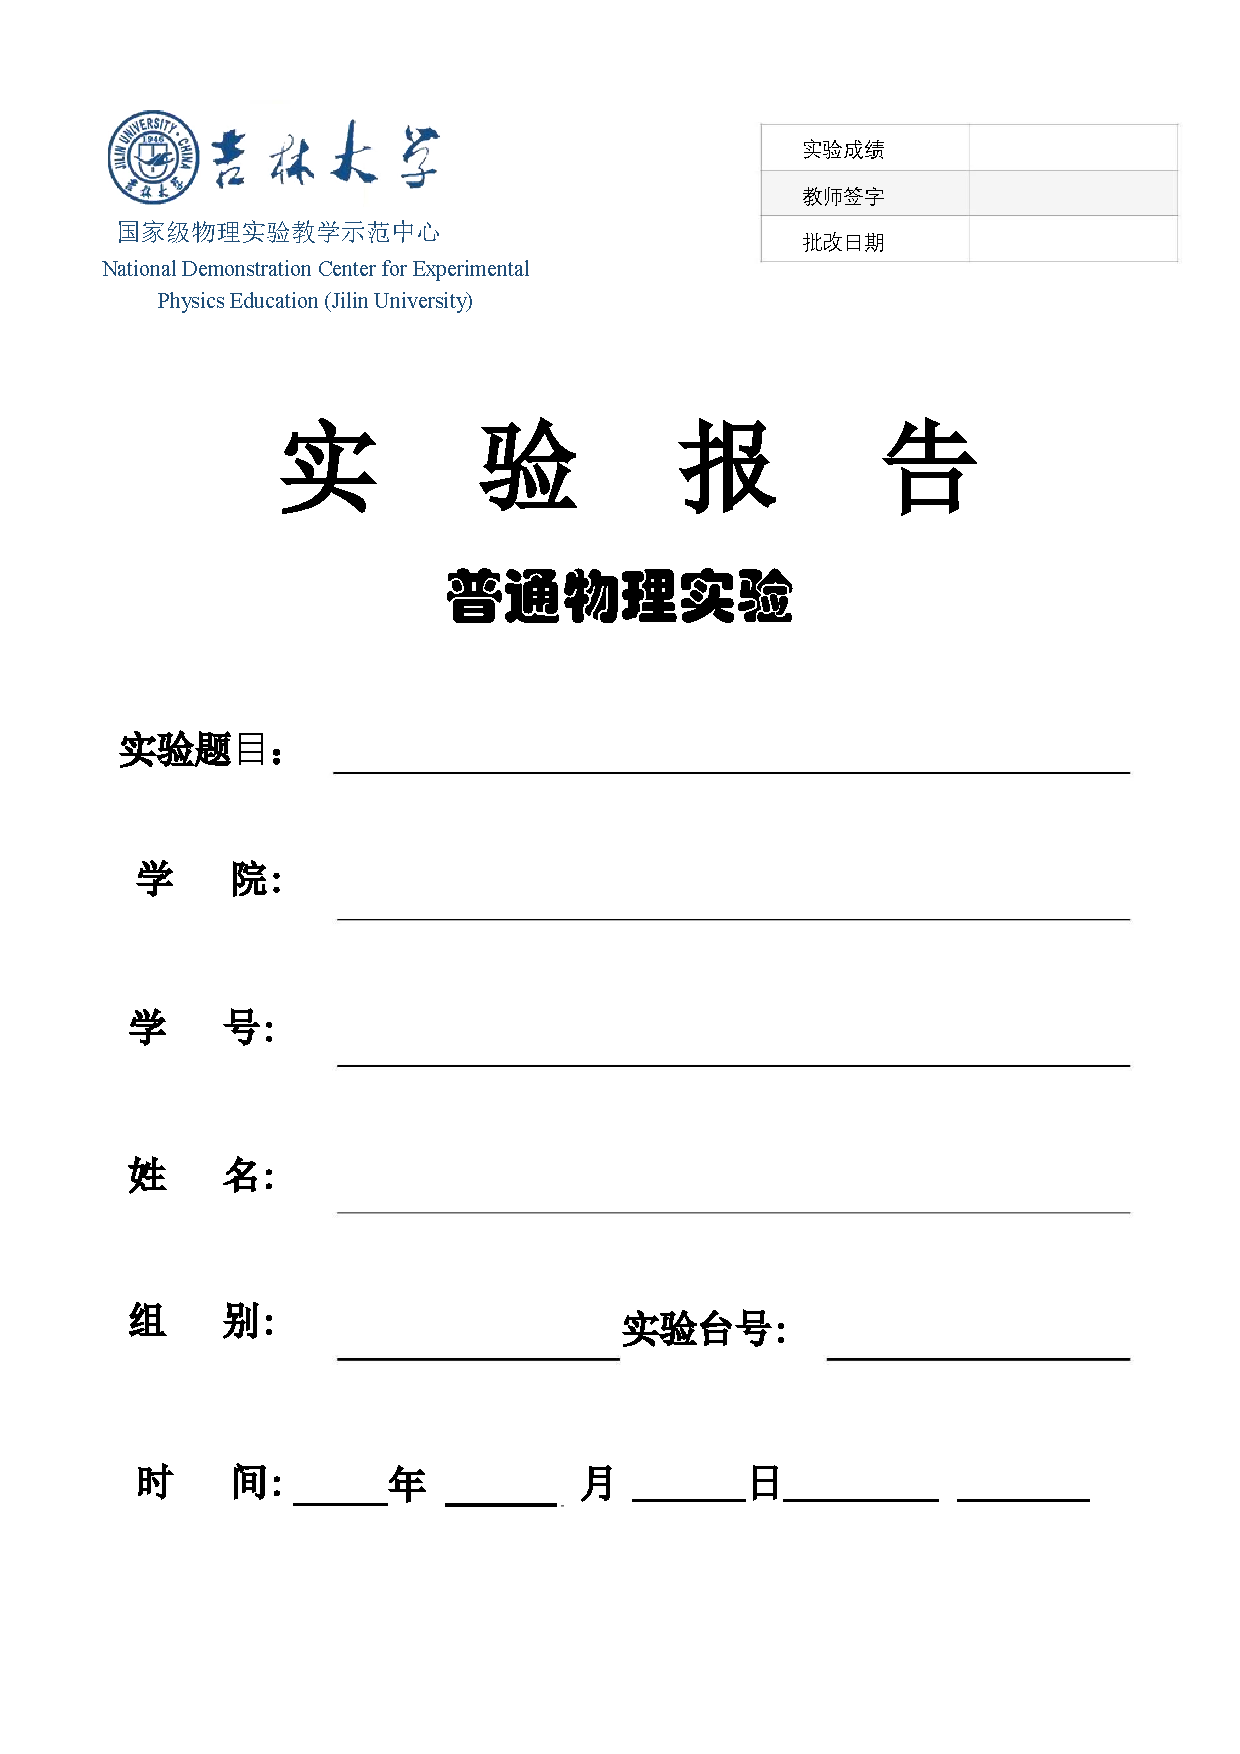
\includepdf[pages=-]{封面.pdf}
\end{titlepage}


\section{实验内容}

\begin{enumerate}
    \item 首先调节将物屏、像屏与凹凸透镜放置在光导轨上,并通过粗调和细调使其共轴
    \item 物像法测凸透镜焦距:使物与像屏之间的距离稍大于4倍焦距,移动待测透镜直至屏呈现清晰的像,同时记录物、像以及透镜位置,计算出焦距f。重复3次求其平均值
    \item 位移法测凸透镜焦距:将物、凸透镜和像屏置于导轨上,调节各元件的主光轴重合,测出物屏与像屏之间的距离 D,移动透镜,使屏得到清晰的像,记录透镜位置,移动透镜至另一位置,使屏上又得到清晰的像,记录透镜位置,测出 d,求出焦距f。固定 D不变,重复3次求平均值
    \item 自准直法测凸透镜焦距:将像屏改为平面镜,调节各元件,调节物距使得物与虚像共面,记录物与透镜间的距离即为待测焦距f。重复3次求平均值
    \item 辅助透镜法测凹透镜焦距:调节物与凸透镜、凹透镜共轴,调节适当位置,使屏上出现清晰的像,记录凹透镜位置和像屏位置,取下凹透镜,调节像屏位置使其呈现清晰的像,记录像屏位置,求出焦距f。重复3次求平均值
    \item 自准直法测凹透镜焦距:将各元件按辅助法中最初所测位置摆放,使屏上出现清晰的像,将屏远离透镜,改变凹透镜位置使屏上重新呈现清晰的像,多次操作使像屏移动足够远,取下像屏,用平面镜靠近凹透镜,使物与清晰的虚像共面,测量两透镜所在位置,作差结果即为焦距f。测量3次求平均值
\end{enumerate}





\section{原始数据}

凸透镜焦距的测量

\begin{table}[H]
\centering
\caption{物像法测凸透镜焦距(单位:cm)}
\begin{tabular}{|c|c|c|c|c|}
\hline
 组别  & 物屏 & 凸透镜 & 像 &  焦距  \\
 \hline
  1   &  120.00 & 101.20 & 79.65 & 10.04 \\
\hline
  2   &  120.00 & 100.51 & 80.12 & 9.96 \\
\hline
  3   &  120.00 & 101.52 & 79.54 & 10.04 \\
\hline
\end{tabular}
\end{table}

\begin{table}[H]
\centering
\caption{位移法测凸透镜焦距(单位:cm)}
\begin{tabular}{|c|c|c|c|c|c|c|c|}
\hline
 组别  & 物屏 & 镜位置1 & 镜位置2  &  像  & D & d & 焦距 \\
 \hline
  1   &  120.00 &  82.91 & 105.72 & 70.01 & 49.99 & 22.81 & 9.90 \\
\hline
  2   &  120.00 &  82.83 & 105.57  &  70.01 & 49.99 & 22.74 & 9.91 \\
\hline
  3   &  120.00 &  82.81 & 105.74  &  70.01  & 49.99 & 22.93 & 9.87\\
\hline
\end{tabular}
\end{table}


\begin{table}[H]
\centering
\caption{自准直法测凸透镜焦距(单位:cm)}
\begin{tabular}{|c|c|c|c|}
\hline
 组别  & 物屏 & 凸透镜 &    焦距  \\
 \hline
  1   &  120.00  & 109.23  & 10.77 \\
\hline
  2   &  120.00 & 109.23 & 10.67 \\
\hline
  3   &  120.00 & 109.28 & 10.72 \\
\hline
\end{tabular}
\end{table}

凹透镜焦距的测量

\begin{table}[H]
\centering
\caption{辅助凸透镜法测凹透镜焦距(单位:cm)}
\begin{tabular}{|c|c|c|c|c|c|}
\hline
 组别  & 凸透镜 & 凹透镜 & 凸像位置 &  凹像位置 & 焦距  \\
 \hline
  1   &  86.32 & 78.02 & 72.94 & 66.53 & -9.11 \\
\hline
  2   &  87.01 & 77.85 & 73.45  & 69.35  & -9.12  \\
\hline
  3   & 86.53 & 77.84 & 72.91  & 67.47  & -9.40  \\
\hline
\end{tabular}
\end{table}


\begin{table}[H]
\centering
\caption{自准直法测凹透镜焦距(单位:cm)}
\begin{tabular}{|c|c|c|c|c|}
\hline
 组别  & 凸透镜 & 凹透镜 & 像屏 &  焦距  \\
 \hline
  1   &  98.52 & 89.83  & 80.34  & -9.29  \\
\hline
  2   &  98.34  & 89.47  & 79.83  &  -9.64  \\
\hline
  3   &  98.77 & 90.03 & 80.87 & -9.16 \\
\hline
\end{tabular}
\end{table}


所测量的数据中导轨刻度的最小分度值为 $ \Delta = 0.1cm$


\newpage

\section{数据处理与分析}

\subsection{物像法测凸透镜焦距不确定度的计算}

以凸透镜位置为原点,则记凸透镜到物屏的距离为负值,到像的距离为正值, 则$\overline{f} = 10.01 \ cm $
\vspace{5cm} %5mm vertical space
% 下述空白处画实验课本上的图

\begin{table}[H]
\centering
\caption{物像法测凸透镜焦距(单位:cm)}
\begin{tabular}{|c|c|c|c|}
\hline
 组别  &  物距 $l$ & 像距 $l'$ & 分度值 $\Delta$   \\
 \hline
  1   &  -18.80 & 21.55  &  \multirow{3}{*}{0.1}  \\
\cline{1-3}
  2   &  -19.49 & 20.39  & \\
\cline{1-3}
  3   &  -18.48 &  21.98  & \\
\hline
均值  &  -18.92 &  21.31 &  \\
\hline
\end{tabular}
\end{table}
根据表格数据计算$A$类测量不确定度如下:
\begin{align*}
    u_A(l) &= \sqrt{
    \frac{\sum_{i=1}^n (l_i - 
    \overline{l})^2}
    {n\times (n-1)}
    }   \\
         &= \sqrt{\frac{(-18.80 + 18.92)^2 +
         (-19.49 + 18.92)^2 +
         (-18.48 + 18.92)^2 }
         { 3\times 2}} \ cm = 0.298 \ cm \\
    u_A(l') &= \sqrt{\frac{\sum_{i=1}^n (l'_i - \overline{l'})^2}{n\times (n-1)}} \\
     &= \sqrt{\frac{(21.55 -21.31 )^2 +
         (20.39 -21.31)^2 +
         (21.98 -21.31)^2 }
         { 3\times 2}} \ cm = 0.475\ cm
\end{align*}
已知其分度值相同,设误差均匀分布 则
\begin{align*}
     u_B(l')  = u_B(l) = \frac{\Delta}{\sqrt{3}} = \frac{0.1}{\sqrt{3}} \ cm= 0.0577 \ cm \\
\end{align*}
其合成标准不确定度
\begin{align*}
    u_c(l) &= \sqrt{u_A(l)^2+u_B(l)^2} = \sqrt{0.298^2 + 0.0577^2} \ cm  = 0.303 \ cm \\
    u_c(l') &= \sqrt{u_A(l')^2+u_B(l')^2} = \sqrt{0.475^2 + 0.0577^2} \ cm = 0.478 \ cm
\end{align*}
由不确定度传递公式
\begin{align*}
    y &= f(x_1,x_2,\dots,x_n) \\
    u_c(y) &= \sqrt{\sum_{i=1}^{n}(\frac{\partial f}{\partial x_i})^2 u^2_{c(x_i)}}
\end{align*}
已知$\frac{1}{f} = \frac{1}{l'} - \frac{1}{f}$,得到 
\begin{align*}
    \frac{u_f}{f} &= \sqrt{ \Big(  \frac{u_c(l')}{l'}  \Big)^2 +
    \Big(  \frac{u_c(l)}{(-l)}  \Big)^2 } \\
    &=  \sqrt{ \Big(  \frac{0.478}{21.31}  \Big)^2 +
    \Big(  \frac{0.303}{18.92}  \Big)^2 } 
\end{align*}
代入 $ f = 10.01 \ cm$ 得到 $ u_f = 0.276 \ cm$。
由 $p=0.955$,对应的置信概率 $K_p=2$。代入上述数据及公式可得其扩展不确定度如下:
\begin{align*}
    U_f = K_p \times u_f = 2 \times 0.276 \ cm = 0.552 \ cm 
\end{align*}
得到焦距的值为 $f = 10.01 \pm 0.552 \ cm$,$p = 0.955$

\subsection{位移法测凸透镜焦距不确定度的计算}
由原始数据得到 焦距均值为 $\overline{f} = 9.89 \ cm$

实际实验中,固定光源(物屏)的位置与像(屏)的位置,故由表格测得数据得到 $D$ 的合成不确定度
\begin{align*}
    u_A(D) &= 0 , \ u_B(D) = \frac{\Delta}{\sqrt{3}} \\
    u_c(D) &=  \sqrt{u_A(D)^2+u_B(D)^2} = u_B(D) = 0.0577 \ cm  
\end{align*}
已知公式
\begin{flalign*}
    l_1 + l'_1 &= D  &\\
    l_1 &= \frac{D-d}{2} & \\
    l'_1 &= \frac{D+d}{2} & \\
\end{flalign*}                          % 空白处画光路图
实验中为了简化步骤减小误差,用位移法测得的实际为成缩小实像和放大实像的凸透镜的实际位置1和位置2,设其值为$l_1$、$l_2$,则$d = l_2 - l_1$ 
\begin{table}[H]
    \begin{tabular}{|c|c|c|c|}
    \hline
      组别   &  $l_1/cm$  & $l_2/cm$  & $d/cm$\\
      \hline
       1  &  82.91 & 105.72  & 22.81\\
       \hline
       2  &  82.83 & 105.57  & 22.74\\
       \hline
       3  &  82.81  & 105.74  & 22.93\\
       \hline
       均值 & 82.85 & 105.68  & 22.83\\
       \hline
    \end{tabular}
    \label{tab:my_label}
\end{table}
根据上述表格计算$l_1$、$l_2$的$A$类统计不确定度如下:
\begin{align*}
    u_A(l_1) &=\sqrt{\frac{\left(\left(82.91-82.85\right)^{2} +
    \left(82.83-82.85\right)^{2} +
    \left(82.81-82.85\right)^{2}\right)}
    {3 \times 2}} \ cm = 0.0306 \ cm \\
    u_A(l_2) &=  \sqrt{\frac{\left(\left(105.72\ -\ 105.68\right)^{2}+\left(105.57\ -\ 105.68\right)^{2}+\left(105.74\ -\ 105.68\right)^{2}\right)}{3 \times 2}} \ cm =  0.0537 \ cm
\end{align*}
已知其分度值相同,设误差均匀分布 则计算
\begin{align*}
     u_B(l_1)  = u_B(l_2) = \frac{\Delta}{\sqrt{3}} = \frac{0.1}{\sqrt{3}} \ cm= 0.0577 \ cm 
\end{align*}
其合成标准不确定度
\begin{align*}
    u_c(l_1) &= \sqrt{u_A(l_1)^2+u_B(l_1)^2} = \sqrt{0.0306^2 + 0.0577^2} \ cm  = 0.065 \ cm \\
    u_c(l_2) &= \sqrt{u_A(l_2)^2+u_B(l_2)^2} = \sqrt{0.0537^2 + 0.0577^2} \ cm = 0.079 \ cm
\end{align*}
由不确定度传递公式
\begin{align*}
    u_c(d) = \sqrt{
    u_c(l_1)^2 + u_c(l_2)^2
    } = \sqrt{0.065^2 + (-0.079)^2} =0.102 \ cm 
\end{align*}
已知 $f = \frac{D^2 - d^2}{4D}$
可得 
\begin{align*}
    u_f &= \sqrt{ \Big( \frac{D^2 + d^2}{4D^2} \Big)^2u_c(D)^2 +
                 \Big( \frac{-d}{2D} \Big)^2u_c(d)^2
    } \\
    &= \sqrt{ \Big( \frac{49.99^2 + 22.83^2}{4 \times 49.99^2} \Big)^2\times 0.0577^2 +
                 \Big( \frac{-22.83}{2 \times 49.99} \Big)^2 \times 0.102^2
    } = 0.029 \ cm 
\end{align*}
得到 $ u_f = 0.029 \ cm$。
由 $p=0.955$,对应的置信概率 $K_p=2$。代入上述数据及公式可得其扩展不确定度如下:
\begin{align*}
    U_f = K_p \times u_f = 2 \times 0.029 \ cm = 0.058 \ cm 
\end{align*}
得到焦距的值为 $f = 9.89 \pm 0.058 \ cm$,$p = 0.955$

\subsection{辅助透镜法测凹透镜焦距不确定度的计算}
由原始数据得到 焦距均值为 $\overline{f} = -9.21 \ cm$   % 空白处画光路图
\begin{table}[H]
\begin{tabular}{|c|c|c|c|}
\hline
 组别  &  $l$ &  $l'$ & 分度值 $\Delta$   \\
 \hline
  1   & 5.08  & 11.49  &  \multirow{3}{*}{0.1}  \\
\cline{1-3}
  2   &  4.40 & 8.50  & \\
\cline{1-3}
  3   &  4.93 &  10.37  & \\
\hline
均值  &  4.80 & 10.12  &  \\
\hline
\end{tabular}
\end{table}
根据上述表格计算$l$、$l'$的$A$类统计不确定度如下:
\begin{align*}
    u_A(l) 
         &= \sqrt{\frac{(5.08 - 4.80)^2 +
         (4.40 - 4.80)^2 +
         (4.93 - 4.80)^2 }
         { 3\times 2}} \ cm = 0.206 \ cm \\
    u_A(l')
     &= \sqrt{\frac{(11.49 - 10.12 )^2 +
         (8.50 - 10.12)^2 +
         (10.37 - 10.12)^2 }
         { 3\times 2}} \ cm = 0.872 \  cm
\end{align*}
已知其分度值相同,设误差均匀分布 则
\begin{align*}
     u_B(l')  = u_B(l) = \frac{\Delta}{\sqrt{3}} = \frac{0.1}{\sqrt{3}} \ cm= 0.0577 \ cm 
\end{align*}
其合成标准不确定度
\begin{align*}
    u_c(l) &= \sqrt{u_A(l)^2+u_B(l)^2} = \sqrt{0.206^2 + 0.0577^2} \ cm  = 0.214 \ cm \\
    u_c(l') &= \sqrt{u_A(l')^2+u_B(l')^2} = \sqrt{0.872^2 + 0.0577^2} \ cm = 0.874 \ cm
\end{align*}
已知公式$\frac{1}{f} = \frac{1}{l'} - \frac{1}{l} $,由不确定度传递公式得到:
\begin{align*}
    \frac{u_f}{f} &= \sqrt{ \Big(  \frac{u_c(l')}{l'}  \Big)^2 +
    \Big(  \frac{u_c(l)}{l}  \Big)^2 } \\
    &=  \sqrt{ \Big(  \frac{0.872}{10.12}  \Big)^2 +
    \Big(  \frac{0.214}{4.80}  \Big)^2 } 
\end{align*}
代入 $ f = -9.21 \ cm$ 得到 $ u_f = -0.894 \ cm$。
由 $p=0.955$,对应的置信概率 $K_p=2$。代入上述数据及公式可得其扩展不确定度如下:
\begin{align*}
    U_f = K_p \times u_f = 2 \times (-0.894) \ cm = -1.788 \ cm 
\end{align*}
得到焦距的值为 $f = -9.21 \pm 1.788 \ cm$,$p = 0.955$

\subsection{自准直法测凸透镜和凹透镜焦距不确定度的计算}
记测凸透镜焦距时凸透镜位置为$x_1$,物屏位置为$x_2$,测得焦距为$f_1$。同时记测凹透镜焦距时像屏位置为$x_3$,凹透镜位置为$x_4$,测得焦距为$f_2$
\begin{table}[H]
\centering
    \begin{tabular}{|c|c|c|c|c|c|c|}
    \hline
      组别   &  $x_1/cm$  & $x_2/cm$  & $f_1/cm$  & $x_3/cm$ & $x_4/cm$  & $f_2/cm$\\
      \hline
       1  &  109.23 & 120.00  & 10.77  & 80.34 & 89.83 & -9.29 \\
       \hline
       2  &  109.23 & 120.00  & 10.67 & 79.83 & 89.47 & -9.64 \\
       \hline
       3  &  109.28  & 120.00  & 10.72 & 80.87 & 90.03 & -9.16 \\
       \hline
       均值 &  109.25  & 120.00  &  10.72 & 80.35 & 89.78 & -9.36 \\
       \hline
    \end{tabular}
    \label{tab:my_label}
\end{table}
\vspace{7cm}% 空白处画光路图
$A$类统计不确定度的计算
\begin{align*}
    u_A(x_1) &=\sqrt{\frac{\left( \left( 109.23-109.25  \right)^{2} +
    \left(109.23-109.25\right)^{2} +
    \left(109.28-109.25\right)^{2}\right)}
    {3 \times 2}} \ cm = 0.0168 \ cm \\
    u_A(x_2) &=  0 \ cm \\
    u_A(x_3) &=\sqrt{\frac{\left( \left( 80.34-80.35  \right)^{2} +
    \left(79.83 - 80.35\right)^{2} +
    \left(80.87 - 80.35\right)^{2}\right)}
    {3 \times 2}} \ cm = 0.3002 \ cm \\
    u_A(x_4) &=\sqrt{\frac{\left( \left( 89.83 - 89.78  \right)^{2} +
    \left( 89.47 - 89.78\right)^{2} +
    \left(90.03 - 89.78\right)^{2}\right)}
    {3 \times 2}} \ cm = 0.1639 \ cm
\end{align*}
已知其分度值相同,设误差均匀分布 则
\begin{align*}
     u_B(x_1)  = u_B(x_2) =  u_B(x_3) =  u_B(x_4) =\frac{\Delta}{\sqrt{3}} = \frac{0.1}{\sqrt{3}} \ cm= 0.0577 \ cm 
\end{align*}
其合成标准不确定度
\begin{align*}
    u_c(x_1) &= \sqrt{u_A(x_1)^2+u_B(x_1)^2} = \sqrt{0.0168^2 + 0.0577^2} \ cm  = 0.060 \ cm \\
    u_c(x_2) &= \sqrt{u_A(x_2)^2+u_B(x_2)^2} = u_B(x_2) = 0.0577 \ cm \\
    u_c(x_3) &= \sqrt{u_A(x_3)^2+u_B(x_3)^2} = \sqrt{0.3002^2 + 0.0577^2} \ cm  = 0.306 \ cm \\
    u_c(x_4) &= \sqrt{u_A(x_4)^2+u_B(x_4)^2} = \sqrt{0.1639^2 + 0.0577^2} \ cm  = 0.174 \ cm 
\end{align*}
对于凸透镜而言,焦距$f_1 = x_2 - x_1$;
对于凹透镜而言,焦距 $f_2 = x_3 - x_4$。
故由不确定度传递公式得到
\begin{align*}
    u_{f_{1}} &= \sqrt{
    u_c(x_1)^2 + u_c(x_2)^2
    } = \sqrt{0.060^2 + 0.0577^2} \ cm = 0.083 \ cm  \\
     u_{f_{2}} &= \sqrt{
    u_c(x_3)^2 + u_c(x_4)^2
    } = \sqrt{0.306^2 + 0.174^2}\ cm= 0.352 \ cm  
\end{align*}
由 $p=0.955$,对应的置信概率 $K_p=2$。代入上述数据及公式可得其扩展不确定度如下:
\begin{align*}
    U_{f_{1}} &= K_p \times u_{f_{1}} = 2 \times 0.083 \ cm = 0.166 \ cm \\
    U_{f_{2}} &= K_p \times u_{f_{2}} = 2 \times 0.352 \ cm = 0.704 \ cm
\end{align*}
得到凸透镜焦距的值为 $f_1 = 10.72 \pm 0.166 \ cm$,$p = 0.955$

凹透镜焦距的值为 $f_2 = -9.36 \pm 0.704 \ cm$,$p = 0.955$


\section{实验结果讨论}
\begin{enumerate}
    \item 物像法测凸透镜焦距得到 $f = 10.01 \pm 0.552 \ cm$,$p = 0.955$ ,误差不符合预期。
    
    推测原因如下:测量 $L$ 和 $L'$时容易对透镜的重心估计不准,在测定使像屏呈现最清晰像时的位置确定不准确,测量出的像屏到透镜间的距离偏大,导致计算得出的焦距误差偏大。
    \item 位移法测凸透镜焦距得到 $f = 9.89 \pm 0.058 \ cm$,$p = 0.955$,误差符合预期
    \item 自准直法测凸透镜焦距得到 $f = 10.72 \pm 0.166 \ cm$,$p = 0.955$,误差在允许范围内,符合预期。
    \item 辅助透镜法测凹透镜焦距,得到 $f = -9.21 \pm 1.788 \ cm$,$p = 0.955$,误差较大不符合预期。
    
    推测原因如下:像屏与凹透镜间的距离选取的比较小,对位置的测量存在细微误差时,对结果的影响就会很大。同时测量凹透镜焦距时难以判别在哪个确切位置成最清晰的像,导致第二次成像点位置的测量与实际情况存在较大误差,本次实验中计算得出凹透镜与第二次成像点的距离偏小,导致计算出的焦距偏大。
    \item 自准直法测凹透镜焦距,得到 $f_2 = -9.36 \pm 0.704 \ cm$,$p = 0.955$,误差偏大不符合预期。
    
    推测原因如下:固定凸透镜后,凸透镜与像的距离较小,导致凹透镜可移动范围过小,故导致测量出现偏差较大,从而误差较大。
\end{enumerate}

\section{实验心得}
经过亲自到实验室进行实验测量薄透镜焦距使我对光路和透镜所呈现的物理现象有了更深刻的了解。实验过程中要注意共轴,并且需要调整平面反射镜以修正过于共轴的现象。同时体会到读取数据与实际采集数据、调整透镜等操作对整体数值的较大影响程度。
\section{思考题}

\subsection{观察成像边缘颜色改变时像距数值的比较}
$l'$更大。由于红光折射率小于紫光,要使成像边缘呈紫光必须靠近透镜。所以边缘呈色波长越小离透镜越近。

\subsection{确定透镜成像正确位置的方法}
调节光具座上的元件,使像“1”中拐角处最清晰即为正确的位置

\subsection{比较各种方法的优缺点}
\begin{enumerate}
    \item 物像法测焦距操作比较简便,但容易因为测量物距与像距时由于对中心估
计不准所带来的误差
    \item 位移法测透镜焦距操作比物像法复杂,但能避免上述误差。
    \item 自准法测透镜焦距操作也简便,但成像不宜判断,其结果受透镜自身结构影
响比较大,从正反两面分别测量后取平均值才能得到较为可靠的数据,否则测得的焦距容易偏大或偏小。
\end{enumerate}
\end{document}